% Licensed to the Apache Software Foundation (ASF) under one or more
% contributor license agreements. See the NOTICE file distributed with
% this work for additional information regarding copyright ownership.
% The ASF licenses this file to You under the Apache License, Version 2.0
% (the ``License''); you may not use this file except in compliance with
% the License. You may obtain a copy of the License at
%
% http://www.apache.org/licenses/LICENSE-2.0
%
% Unless required by applicable law or agreed to in writing, software
% distributed under the License is distributed on an ``AS IS'' BASIS,
% WITHOUT WARRANTIES OR CONDITIONS OF ANY KIND, either express or implied.
% See the License for the specific language governing permissions and
% limitations under the License.

\subsubsection{Web Crawler Job Options}

You must fill in six more tabs to configure a Web Crawler job.

\bigimage{web-edit-job-tab3}

\ifJDBCGuide
% Licensed to the Apache Software Foundation (ASF) under one or more
% contributor license agreements. See the NOTICE file distributed with
% this work for additional information regarding copyright ownership.
% The ASF licenses this file to You under the Apache License, Version 2.0
% (the ``License''); you may not use this file except in compliance with
% the License. You may obtain a copy of the License at
%
% http://www.apache.org/licenses/LICENSE-2.0
%
% Unless required by applicable law or agreed to in writing, software
% distributed under the License is distributed on an ``AS IS'' BASIS,
% WITHOUT WARRANTIES OR CONDITIONS OF ANY KIND, either express or implied.
% See the License for the specific language governing permissions and
% limitations under the License.

\begin{itemize}
\label{scheduling}

\item \textbf{Schedule type:} Whether you want to scan every document
once or dynamically recrawl content in your repository. 

When scanning every document once, the crawler marks all documents that
have been previously crawled in this job as potentially to be deleted,
adds all seed documents to its queue and marks them as pending, processes
pending documents, marking them completed as they are ingested, and then
deleted all of the documents that were not recrawled. A document might
not be recrawled because it no longer exists, or the job specification
might have been changed to no longer include the document.

When dynamically recrawling documents, the crawler does not start by
marking all documents as potentially deletable; instead, it begins with
all of the seed documents, and continues adding to its list, periodically
re-adding the initial seed documents. If a document is removed from the
source, it will expire in the expiration interval (see below).

\item \textbf{Expiration Interval (if continuous):} The length of the
interval (in minutes) that the appliance will retain a document
crawled by this job after the document no longer appears in the
repository. After this interval, the missing document will be removed
from the appliance's index and archive. Leave the expiration interval
blank to keep missing documents indexed in GTS.

\item \textbf{Recrawl interval:} If you are dynamically recrawling
documents, how long, in minutes, the crawler should wait before
crawling documents a second time.

\item \textbf{Reseed interval:} If you are dynamically recrawling
documents, how long, in minutes, the crawler should wait before
looking for new documents to crawl. \ifMeridioGuide This connector
identifies all documents for ingestion through seeding; if the reseed
interval is infinite, the job will not ingest documents placed in the
repository during run time. (The job automatically reseeds whenever it
is started.) The default interval of 60 minutes is an appropriate
reseed rate. \fi \ifFilenetGuide This connector identifies documents
for ingestion during seeding. If you change the document inclusion
criteria, reseeding is required to identify new documents. Similarly,
documents placed in the repository while the job is running will not
be identified until the crawl is reseeded.  (The job automatically
reseeds whenever it is started.) The default interval of 60 minutes is
an appropriate reseed rate. \fi

\item \textbf{Scheduled time:} Allows you to define a time you wish
the job to run using a series of selection boxes. The first box refers
to the day of the week you wish the job to run, with an option to have
the job run any day of the week. The second box allows you to select
the start hour, with an option to start the job at any hour. The third
box allows you to specify which minute after the hour that you wish
the job to start. The fourth box allows you to specify what months of
the year you wish the job to run, with an option for the job to run
any month. The last box allows you to specify the day of the month you
wish the job to start, including any day of month.


You can scroll through each of the five boxes in this setting using
the arrow keys on your keyboard or by using the scroll bar on the
right side of the box.  If you want to select more than one value,
hold down control as you scroll and click the values that you want to
select. This allows you to define multiple windows with the same
length, for example by selecting Monday, Wednesday, and Friday at the
same time.

\item \textbf{Maximum run time:} The longest you will allow the job to
run, in minutes. For example, if you want to start a job at 2 AM but
force it to stop at 8 AM so that users have access to the repository,
you should set this value to 360 minutes. If the job is not complete by the
end time, documents that have already been found will be indexed, and
the rest of the crawl will continue at the beginning of the next
schedule interval. 

When you have defined the scheduled time and assigned a maximum run
time, click on the ``Add Scheduled Time'' button. A new schedule box
will appear below the scheduled time, allowing you to create
additional scheduled run times.

Here is a sample schedule for a job that will run every
Monday from 2 am to 6 am:

\begin{changemargin}{-.3in}{0in} 
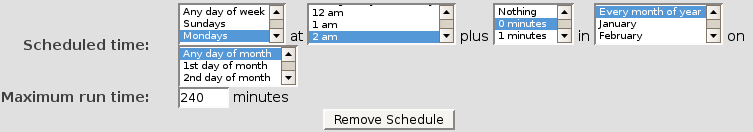
\includegraphics[width=300pt]{sample-schedule}
\end{changemargin}

If you do not have at least one scheduled time, the job will
only run when run manually (see page \pageref{ManageJobs}), and will
not automatically update the index on the appliance based on changes
to the repository.

You can remove a scheduled time by clicking the ``Remove Schedule''
button.

\end{itemize}

\fi

\ifCombinedConnectorGuide
This tab presents scheduling options. Here you can generate one or
more scheduled run times for the job. For a complete description of
the scheduling options, see the description starting on page
\pageref{scheduling}.
\fi

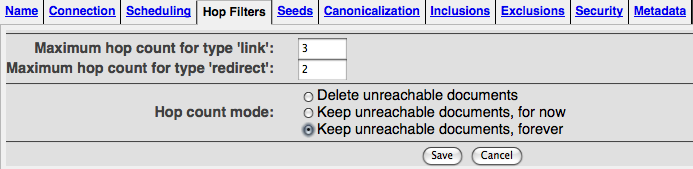
\includegraphics[width=300pt]{web-edit-job-tab4}

\begin{itemize}

\item \textbf{Maximum hop count for type 'link':} The web crawler begins
at the seed documents provided on the following tab, and follows links
in the bodies of the documents, if applicable.  Only documents where
the crawler follows this number or fewer links to reach that document
from a seed document will be processed.


\item \textbf{Maximum hop count for type 'redirect':} The maximum hop
count for type 'redirect' limits which documents will be processed by
the crawl based on the number of redirect links between that document
and a seed document.

\item \textbf{Hop count mode:} Documents may become unreachable within the
limiting number of hops from the seed documents. This setting determines
how documents that become unreachable are treated in the database.

\begin{itemize}

\item \textbf{Delete unreachable documents}:
Documents that become unreachable from the seed pages in the number of
hops specified above will be deleted from the database. Deleting
unreachable documents may affect resources available on the appliance.

\item \textbf{Keep unreachable documents, for now}:
When the crawler attempts to re-crawl a document and finds it
unreachable, the documents are kept. You can decide at any point later
to keep these documents forever or to delete them, by changing this
setting. Some appliance resources will be used to maintain the status
of these documents.

% What kinds of resources? Disk? RAM? Sheep?

\item \textbf{Keep unreachable documents forever}:
Documents that are unreachable are kept in the document index. You
cannot delete these documents from the index without deleting the job
used to crawl the documents. This is the preferred setting.

\end{itemize}

\end{itemize}


\bigimage{web-edit-job-tab5}

On this tab, you are presented with a text box into which you should
enter the URLs of the web pages you wish this job to crawl. Each
should be on a separate line of the text box.

\bigimage{web-edit-job-tab6}

This tab allows you to apply some built-in canonicalization tools
to URLs before they are send to the MetaCarta ingestion system. If
canonicalization is not done properly, you risk either having duplicate
copies of the same document (for example, from having arguments to
a script in a different order but calling the script with the same
arguments) or having no copies of a document at all (for example, from
reordering the script arguments in a way that breaks the site being
crawled). The Connector Framework handles the reordering automatically,
but requires your intervention to decide which sites need to be reordered
and which do not.

You can canonicalize based on regular expression; for more information on
regular expressions, please see the explanation in the next tab. Enter
a regular expression, a description of the URL (for your records only),
and then choose the types of canonicalization you would like enabled. You
have the following canonicalization options:

\begin{itemize}

\item \textbf{Reorder}: Take all arguments to any query in the URL and
order them programmatically. For example, a URL might include a query
string like ``article=foo0011\&format=fulltext.'' If the query string
were instead ``format=fulltext \&article=foo0011,'' the MetaCarta system
would treat it as a different document but it would contain the same
information. Normally, we recommend that you reorder all URLs, but
some sites require a specific order; for those sites, you should turn
reordering off.

\item \textbf{Remove JSP sessions}: Most of the time, you can safely
remove JSP session information from URLs. Uncheck this box if you find
that a particular site requires that you leave JSP session information
in the URL.

\item \textbf{Remove ASP sessions}: Most of the time, you can safely
remove ASP session information from URLs. Uncheck this box if you find
that a particular site requires that you leave ASP session information
in the URL.

\item \textbf{Remove PHP sessions}: Most of the time, you can safely
remove PHP session information from URLs. Uncheck this box if you find
that a particular site requires that you leave PHP session information
in the URL.

\item \textbf{Remove BV sessions}: Most of the time, you can safely
remove BV session information from URLs. Uncheck this box if you find
that a particular site requires that you leave BV session information
in the URL.

\end{itemize}

By default, all URLs are canonicalized in all five ways.

\bigimage{web-edit-job-tab7}


Here you can create regular expression matches that will determine
what the crawler includes for ingestion based on URL.  Place each
inclusion expression on a new line in the text box.

The default expression, \texttt{.*}, includes all documents. If you
are crawling the open Internet, this may cause your crawl to follow
links from and ingest many undesirable documents. A better strategy
may be to create expressions that match individual servers or
domains. In the example above, the given match expression\linebreak
\texttt{\^{}https?://[\^{}$\backslash\backslash\backslash$?/]*.example.com} only matches documents from the\linebreak \texttt{example.com} domain.

\note{If you are not familiar with regular expressions, there
are a variety of tutorials available on the web, including
\url{http://gnosis.cx/publish/}\linebreak\url{programming/regular_expressions.html}
and \url{http://perldoc.}\linebreak\url{perl.org/perlrequick.html}. If you still have
difficulty with these settings, please contact Customer Support (see
page \pageref{SupportContact}).}


\bigimage{web-edit-job-tab8}


Here you can create regular expression matches that will determine
what the crawler excludes from ingestion. Place each exclusion
expression on a new line in the text box.

The default blank expression does not exclude any documents. Other
possiblities include specifying specific servers or domains to
exclude. For example, the match expression
\texttt{\^{}https?://media.example.com} excludes any documents from
the \texttt{media.example.com} server. Another possibility is to
exclude files based on file extension. For example, the match
expression \texttt{$\backslash$.exe($\backslash$?|\$)} will exclude any
file with a \texttt{.exe} extension.


\bigimage{web-edit-job-tab9}



\begin{itemize}

\item \textbf{Access Tokens:} If you wish to create ACLs for files
ingested through this job, you can enter access tokens here. Simply
enter one or more ACL identifiers into the field and click the ``Add''
button. The ACL identifiers will appear in a list. You can continue to add
more ACL identifiers using the ``Add'' button, or remove them using the
``Delete'' button that appears next to each ACL identifier. By default,
documents ingested through the Web Crawler will be accessible to all
authorized search users. For assistance with this configuration, contact
MetaCarta Support (see page \pageref{SupportContact}).

%% don't we explain this in other guides? It would be nice to explain it, I think... 

\end{itemize}


\bigimage{web-edit-job-tab10}


\begin{itemize}

\item \textbf{Metadata:} Here you can add additional metadata to be ingested along with documents crawled by this job. You should not overwrite existing metadata fields, such as collection name, using this tool.

\end{itemize}

After entering this information, you will be taken to the status page
for this job:

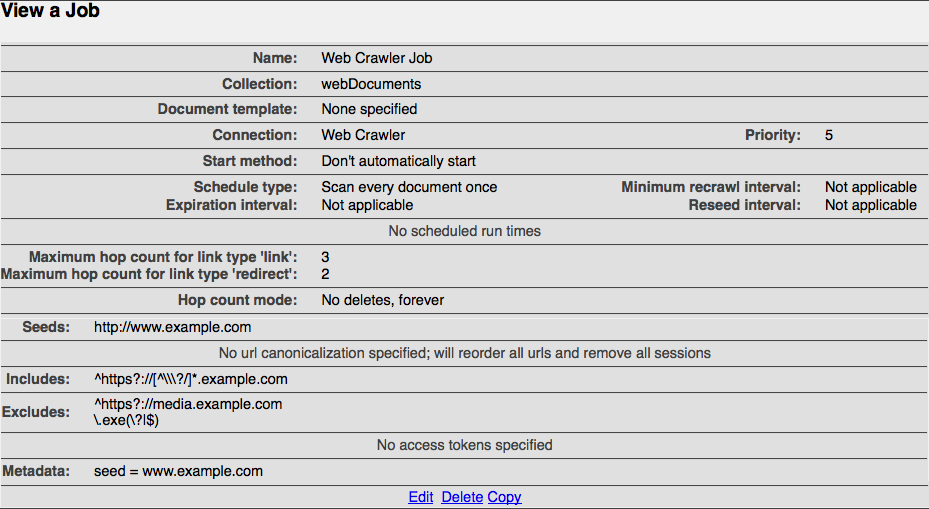
\includegraphics[width=300pt]{web-view-job-status}
